\documentclass[12pt]{article}
\usepackage{caption}
\usepackage{xcolor}
\usepackage{setspace}
\usepackage{makecell}
\usepackage{tabu}
\usepackage{colortbl}
\usepackage{longtable}
\usepackage[utf8]{inputenc}
\usepackage{url}
\usepackage[top=30mm, bottom=20mm, left=30mm, right=20mm]{geometry}
\usepackage{pdflscape}
\usepackage{float}
\usepackage{array, longtable}

\newcommand{\cbox}[2][yellow]{%
  \colorbox{#1}{\parbox{\dimexpr\linewidth-2\fboxsep}{\strut #2\strut}}%
}

\renewcommand\theadalign{bc}
\renewcommand\theadfont{\bfseries}
\renewcommand\theadgape{\Gape[4pt]}
\renewcommand\cellgape{\Gape[4pt]}
\newcommand\tab[1][1cm]{\hspace*{#1}}

\onehalfspacing

\begin{document}

    \begin{center}

\begin{Large}
    \textbf{CENTRO FEDERAL DE EDUCAÇÃO TECNOLÓGICA DE MINAS GERAIS }
\end{Large}

\vspace{0.5cm}

\begin{normalsize}
    \textbf{CAMPUS TIMÓTEO}
\end{normalsize}

\vspace{5cm}

\begin{Huge}

    % Título do arquivo
    \textbf{Documentação de desenvolvimento de projeto de software}
    
    \vspace{0.5cm}
    
    % Nome do projeto
   \textbf{ {\color{red}[ Nome do projeto ]}}
    
\end{Huge}

\vspace{5cm}

\textbf{Aluno: } {\color{red} [ Nome do(a) aluno(a) ]}

\vspace{0.5cm}

\textbf{{\color{red}TURNO/TURMA}}

\vspace{2cm}

Timóteo - MG

\vspace{1cm}

{\color{red} [ dia ]} de {\color{red} [ mês por extenso ] } de {\color{red} [ ano com 4 dígitos ] }

\end{center}

\newpage
    
    \section{Glossário}

\noindent \cbox{
   Todas as siglas e termos próprios do negócio.
}


\textbf{API} - Application Programming Interface (Interface de programação para aplicações);

...
   


    \section{Materiais de referência}

\noindent \cbox{
    Todos os materiais e documentos que servem de referência para os requisitos e os modelos do projeto – seguem alguns exemplos abaixo
}

\begin{center}
    
    \begin{longtable}{|p{4cm}|p{11.5cm}|}
        
        \hline
        
        \textbf{Tipo de material} & 
        \textbf{Referência} \endhead    
        
        \hline

        Atas de entrevistas & 
        Entrevistas realizadas com funcionários da empresa na data ... \\ \hline
        
        
        Documento & 
        Ficha de cadastro de cliente \\ \hline
        
        
        Relatório & 
        Plano do projeto \\ \hline
        
        ... & 
        ... \\ \hline
    
    \end{longtable}
    
    \captionof{table}{Tabela de materiais de referência. Fonte: autores.}
    
\end{center}

    \section{Descrição do minimundo do projeto}

\noindent \cbox{
    Repetir aqui o minimundo já aprovado na proposta e mantê-lo sempre atualizado.
}

    \section{Descrição dos atores}

\begin{center}
    
    \begin{longtable}{|p{1cm}|p{2cm}|p{5cm}|p{3cm}|p{4cm}|}
    
        \hline
    
        \textbf{Nº} &
        \textbf{Nome} &
        \textbf{Descrição} &
        \textbf{Frequência de uso}  &
        \textbf{Proeficiência em informática} \endhead 
        
        \hline
        
        1 &
        Admin &
        Os administradores são os usuários que têm acesso ao módulo administrativo. Eles têm como objetivo realizar tarefas de característica gerencial, como por exemplo cadastro de novas lojas, consultar dados estatísticos a respeito do sistema, etc. &
        Diária &
        Alta \\ \hline
        
        ... & 
        ... &
        ... &
        ... &
        ... \\ \hline
    
    \end{longtable}
    \captionof{table}{Tabela de descrição dos atores. Fonte: autores.}
\end{center}
    
    \section{Lista de funções do projeto}

\definecolor{cinza_claro}{RGB}{243,243,243} 

\noindent\cbox{
    Repetir aqui a lista já aprovada na proposta e mantê-la sempre atualizada acrescentando novas funcionalidades.
}

\begin{center}
%\begin{longtable}{p{4cm}|l|l|l|l}
\begin{longtable}{|p{1.2cm}|p{4.2cm}|p{5.4cm}|p{1.3cm}|p{1.5cm}|}

    \caption[Lista de funcionalidades do software]{Lista de funcionalidades do software.}
    
    \label{tab:lista_funcionalidades}
    
    \hline  
        \textbf{Núm.} \cellcolor{cinza_claro} &
        \textbf{Nome} \cellcolor{cinza_claro} &
        \textbf{Descrição} \cellcolor{cinza_claro} &
        \textbf{Tipo}  \cellcolor{cinza_claro} &
        \textbf{Atores} \cellcolor{cinza_claro}\\ \hline 
    \endfirsthead
    
    \multicolumn{5}{c}%
    {{\bfseries \tablename\ \thetable{} -- continuação da página anterior}} \\
    \hline 
        \textbf{Núm.} \cellcolor{cinza_claro} &
        \textbf{Nome} \cellcolor{cinza_claro} &
        \textbf{Descrição} \cellcolor{cinza_claro} &
        \textbf{Tipo}  \cellcolor{cinza_claro} &
        \textbf{Atores} \cellcolor{cinza_claro}\\ \hline 
    \endhead
    
    \hline \multicolumn{5}{|r|}{{Continua na próxima página}} \\ \hline
    \endfoot
    
    
    \endlastfoot
        1  & 
        Cadastro & 
        Cadastro de usuários do sistema & 
        3 & 
        3 \\ \hline
        
        
        2  & 
        Login  & 
        Controle de acesso dos atores & 
        3 & 
        1, 2, 3 \\ \hline
        
        
        3  &
        ... & 
        ... & 
        ... & 
        ... \\ \hline
        
        
        

\hline \multicolumn{5}{l}{Fonte: Elaborada pelos autores.}

\end{longtable}
\end{center}


\vspace{0.5cm}

Legenda:


\begin{center}
    \begin{minipage}{0.4\textwidth}
        \centering
        \captionof{table}{Tipos de funcionalidades.}
        \begin{tabular} { | l | l |}
            \hline
            \textbf{Tipo} \cellcolor{cinza_claro} & \textbf{Nome}  \cellcolor{cinza_claro}   \\ \hline
            1              & Entrada de dados   \\ \hline
            2              & Saída de dados     \\ \hline
            3              & Controle de acesso \\ \hline
            4              & Controle           \\ \hline
        
            \multicolumn{2}{l}{Fonte: Elaborada pelos autores.}
        \end{tabular}
    \end{minipage}
    \hspace{1cm}
    \begin{minipage}{0.4\textwidth}
        \centering
        \captionof{table}{Atores do sistema.}
        \begin{tabular} { | l | l |}
            \hline
            \textbf{Número}  \cellcolor{cinza_claro} & \textbf{Nome} \cellcolor{cinza_claro} \\ \hline
            1                       & Gerente            \\ \hline
            2                       & Funcionário        \\ \hline
            3                       & Cliente            \\ \hline
            4                       & Sistema            \\ \hline
            
            \multicolumn{2}{l}{Fonte: Elaborada pelos autores.}
        \end{tabular}
    \end{minipage}
\end{center}

    
    \section{Diagramas e detalhamentos}

    \subsection{Diagrama de casos de uso}

    \noindent \cbox{
        Acrescentar o diagrama de casos de uso
    }
    
    \subsection{Requisitos Funcionais}

    \noindent \cbox{
        Devem ser documentadas todas as funções relacionadas aos casos de uso.
    }
    
    \subsection{Requisitos não Funcionais}

    \noindent \cbox{
        Devem ser documentadas todas as funções relacionadas aos requisitos não funcionais.
    }
    
    \subsection{Diagrama de classes}

    \noindent \cbox{
        Construa o diagrama de classes do seu sistema
    }
    
    \subsection{Diagrama de sequência}

    \noindent \cbox{
        - Desenvolver o Diagrama de Sequência de uma funcionalidade de Cadastro. \\
        - Todas as Funcionalidades de Controle deverão ser acompanhadas dos Diagramas de Sequência correspondentes. \\
        - Desenvolver o Diagrama de Sequência de um relatório
    }
    
    \section{\textbf{Modelo de análise - Projeto de Dados}}
   
\subsection{\textbf{DER (Diagrama Entidade Relacionamento)}}

\noindent \cbox{
     Colocar aqui o DER do seu projeto. Ele pode ser elaborado em ferramentas de modelagem UML ou gerados pelo ambiente de desenvolvimento. (Deve existir em todos os projetos que envolvem banco de dados). O exemplo abaixo é para vocês lembrarem como é.
}
   
\begin{figure}[H]
    \centering
    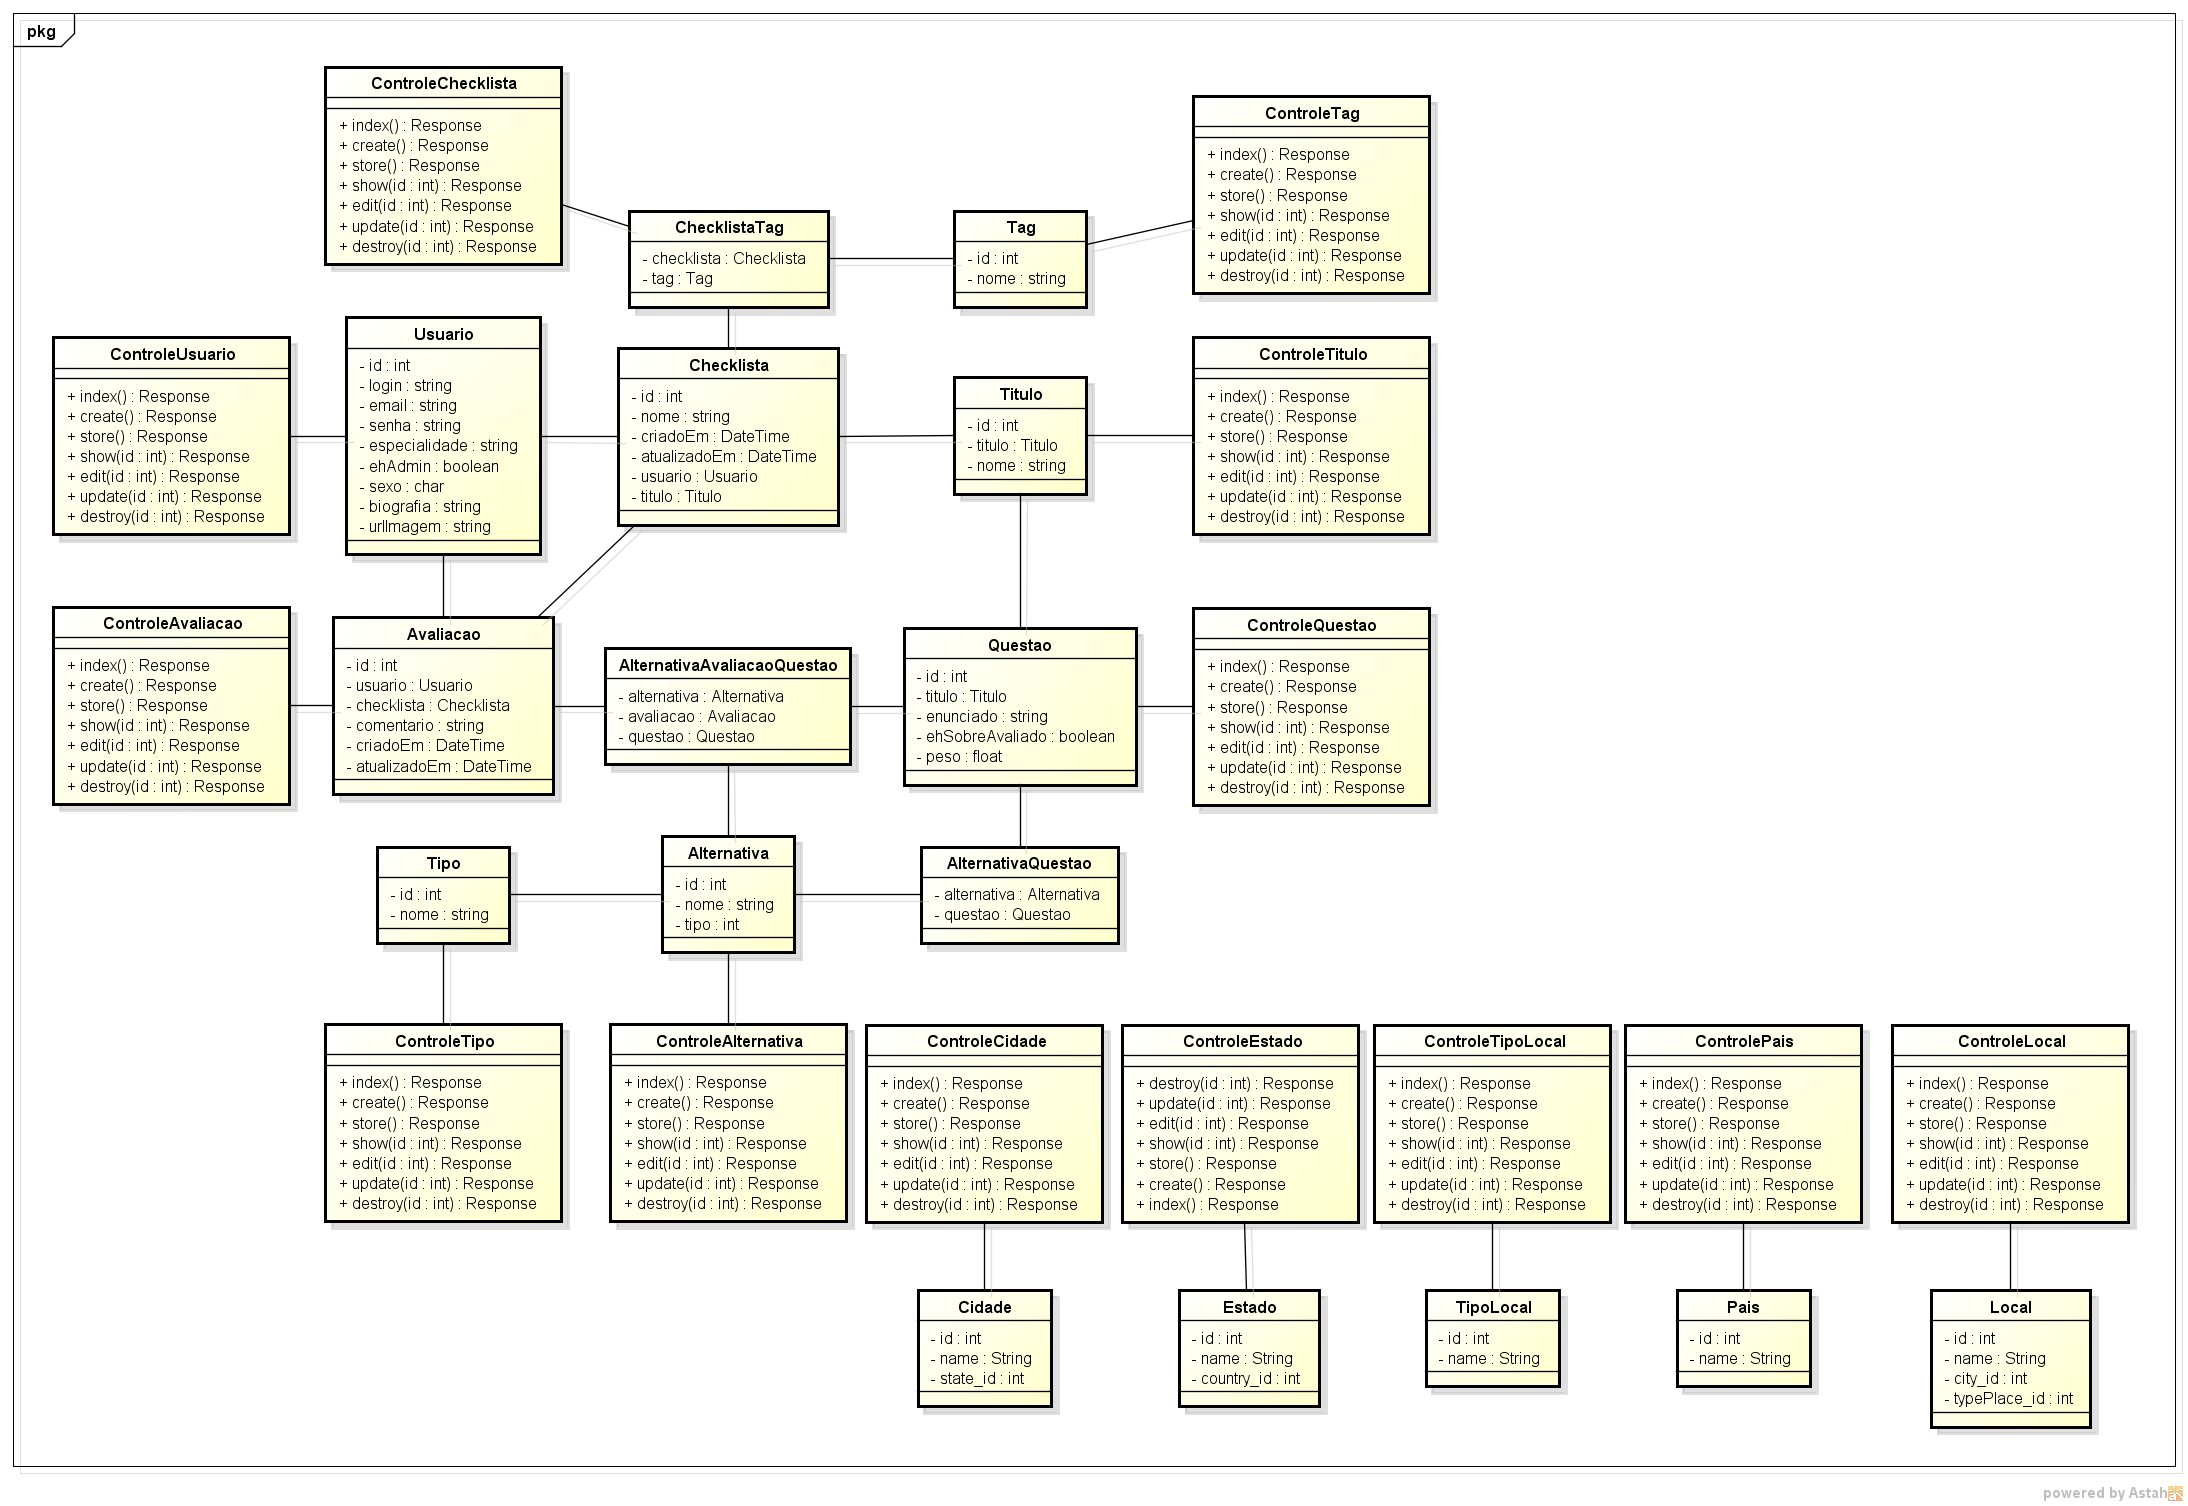
\includegraphics[scale=.3]{imgs/DER.png}
    \label{fig:my_label}
\end{figure}



\begin{landscape}
\subsection{\textbf{Dicionário de dados completo}}

\noindent \cbox{
    Faça um dicionário completo. O exemplo abaixo é para vocês lembrarem como é.
}

\begin{longtable}{|p{3.5cm}|p{1cm}|p{2cm}|p{6cm}|p{2cm}|p{2cm}|p{2cm}|p{2cm}|p{2.5cm}|}
\hline 
\multicolumn{3}{|l|}{ \cellcolor{lightgray} \textbf{Entidade}} & \multicolumn{6}{c|}{ \cellcolor{lightgray}} \\ \hline
\multicolumn{3}{|l|}{\textbf{Nome}} & \multicolumn{6}{l|}{Tabela de Curso} \\ \hline
\multicolumn{3}{|l|}{\textbf{Nome Abreviado}} & \multicolumn{6}{l|}{TbCurso} \\ \hline
\multicolumn{3}{|l|}{\textbf{Índices}} & \multicolumn{2}{l|}{Nome do Índice} & \multicolumn{2}{l|}{Atributos} & \multicolumn{2}{l|}{Único (Sim, Não)}\\ \hline
\multicolumn{3}{|l|}{} & \multicolumn{2}{l|}{IND\_TBCURSO\_NMCURSO} & \multicolumn{2}{l|}{NMCURSO} & \multicolumn{2}{l|}{Sim}\\ \hline
\multicolumn{3}{|l|}{} & \multicolumn{2}{l|}{} & \multicolumn{2}{l|}{} & \multicolumn{2}{l|}{}\\ \hline
\multicolumn{3}{|l|}{\textbf{Descrição}} & \multicolumn{6}{l|}{Tabela que contém todos os cursos oferecidos pela Universidade Miranda.}\\ \hline
\multicolumn{9}{|l|}{ \cellcolor{lightgray} \textbf{Atributos}} \\ \hline

\cellcolor{lightgray} {Nome do Atributo} &  \cellcolor{lightgray} {Tipo} &  \cellcolor{lightgray} {Tamanho} &  \cellcolor{lightgray} {Descrição} &  \cellcolor{lightgray} {Máscara} &  \cellcolor{lightgray} {Regra Validação} &  \cellcolor{lightgray} {Valores Válidos} &  \cellcolor{lightgray} {Range} &  \cellcolor{lightgray} {Integridade Referencial} \\ \hline

CDCURSO &  N & 5,0 & Código do Curso & 99.999 & $>$ 0 & & & \\ \hline
NMCURSO &  T & 50 & Nome do Curso & & Obrigatório & & & \\ \hline
CDAREA & N & 5,0 & Código da Área & 99.999 & $>$ 0 & & & TBAREA \\ \hline
DTINCREG & D & 10 & Data Inclusão Registro & 99/99/9999 & $<=$  date ( ) & & & \\ \hline
CDUSUINC &  N & 5,0 &Código Usuário Incluiu Registro & 99.999 & $>$ 0 &
& & TBUSUARIO \\ \hline
DTALTREC & D & 8 & Data Alteração do Registro &  99/99/9999 & $<=$  date ( ) & & & \\ \hline
CDUSUALT &  N &  5,0 & Código Usuário Alterou  Registro & 99.999 & $>$ 0 & & & \\ \hline
\end{longtable}  

\end{landscape}

\end{document}